% =============================================================================
% Presentacion para asesor doctoral
% Autor: Eric Torres (PUCP)
% Estilo: blanco y negro, sobrio, academico
% =============================================================================

\documentclass[10pt, aspectratio=169]{beamer}

% Tema: minimalista, blanco y negro
\usetheme{default}
\usecolortheme{seagull}        % Paleta gris (sin colores)
\useinnertheme{rectangles}      % Bullets cuadrados, sin sombras
\useoutertheme{miniframes}      % Footer con secciones
\setbeamercovered{transparent}  % Items futuros transparentes

% Forzar blanco y negro: sobreescribir cualquier color residual
\setbeamercolor{normal text}{fg=black, bg=white}
\setbeamercolor{structure}{fg=black}
\setbeamercolor{alerted text}{fg=black}
\setbeamercolor{example text}{fg=black}
\setbeamercolor{frametitle}{fg=black, bg=white}
\setbeamercolor{title}{fg=black, bg=white}
\setbeamercolor{section in head/foot}{fg=black, bg=white}
\setbeamercolor{subsection in head/foot}{fg=black, bg=white}
\setbeamercolor{author in head/foot}{fg=black, bg=white}
\setbeamercolor{title in head/foot}{fg=black, bg=white}
\setbeamercolor{date in head/foot}{fg=black, bg=white}
\setbeamercolor{footline}{fg=black, bg=white}
\setbeamercolor{itemize item}{fg=black}
\setbeamercolor{itemize subitem}{fg=black}
\setbeamercolor{enumerate item}{fg=black}
\setbeamercolor{block title}{fg=white, bg=black}
\setbeamercolor{block body}{fg=black, bg=white}

% Sin sombras, sin gradientes
\setbeamertemplate{blocks}[default]
\setbeamertemplate{itemize items}[square]
\setbeamertemplate{navigation symbols}{}  % Sin barra de navegacion
\setbeamertemplate{footline}[frame number]

% Tipografia
\usefonttheme{serif}
\usepackage[utf8]{inputenc}
\usepackage[T1]{fontenc}
\usepackage[spanish, es-tabla, es-noindentfirst]{babel}
\usepackage{lmodern}
\usepackage{microtype}

% Matematicas
\usepackage{amsmath, amssymb, mathtools}
\usepackage{dsfont}

% Graficos
\usepackage{graphicx}
\graphicspath{{../figures/descriptive/}{../figures/}}

% Tablas
\usepackage{booktabs}
\usepackage{tabularray}
\UseTblrLibrary{booktabs}

% Hyperref sin colores chillones
\usepackage{hyperref}
\hypersetup{
  colorlinks=true,
  linkcolor=black,
  citecolor=black,
  urlcolor=black,
  pdfborderstyle={/S/U/W 0}
}

% Bibliografia (APA 7, mismo .bib que el paper)
\usepackage{csquotes}
\usepackage[backend=biber,
            style=apa,
            natbib=true,
            uniquename=false,
            uniquelist=true,
            sortcites=true,
            maxcitenames=2,
            mincitenames=1,
            maxbibnames=99,
            minbibnames=99,
            giveninits=false]{biblatex}
\DeclareLanguageMapping{english}{english-apa}
\addbibresource{../Bibliography_base.bib}

% =============================================================================
% Metadata
% =============================================================================
\title[Impacto laboral de la IA generativa en ALC]
      {El Impacto Laboral de la Inteligencia Artificial Generativa\\
       Evidencia Causal para América Latina}
\subtitle{Presentación al asesor}
\author{Eric Torres}
\institute{Pontificia Universidad Católica del Perú\\Programa Doctoral en Economía}
\date{\today}

% =============================================================================
\begin{document}

% --- Slide 1: Portada -------------------------------------------------------
\begin{frame}[plain]
  \titlepage
\end{frame}

% --- Slide 2: Plan de la presentacion ---------------------------------------
\begin{frame}{Plan de la presentación}
  \tableofcontents
\end{frame}

% =============================================================================
\section{Motivación y pregunta de investigación}
% =============================================================================

% --- Slide 3: La pregunta ---------------------------------------------------
\begin{frame}{La pregunta}
  \textbf{¿Cómo ha afectado la IA generativa al mercado laboral en América Latina?}
  \vfill
  \begin{itemize}
    \setlength\itemsep{0.6em}
    \item ChatGPT (nov.\ 2022) es el shock tecnológico más comentado de la década.
    \item Las primeras estimaciones causales rigurosas son llamativas: \citet{HumlumVestergaard2025_llm} encuentran efectos sobre salarios y horas \emph{menores al 2\%} en Dinamarca.
    \item Casi toda la evidencia causal disponible viene de la OCDE (Estados Unidos, Dinamarca, plataformas de \emph{freelance}).
    \item Para los países en desarrollo, y en particular para América Latina, no existe estimación causal a la fecha.
  \end{itemize}
\end{frame}

% --- Slide 4: El shock llego a la region (Figura 1) -------------------------
\begin{frame}{El shock llegó a la región}
  \begin{center}
    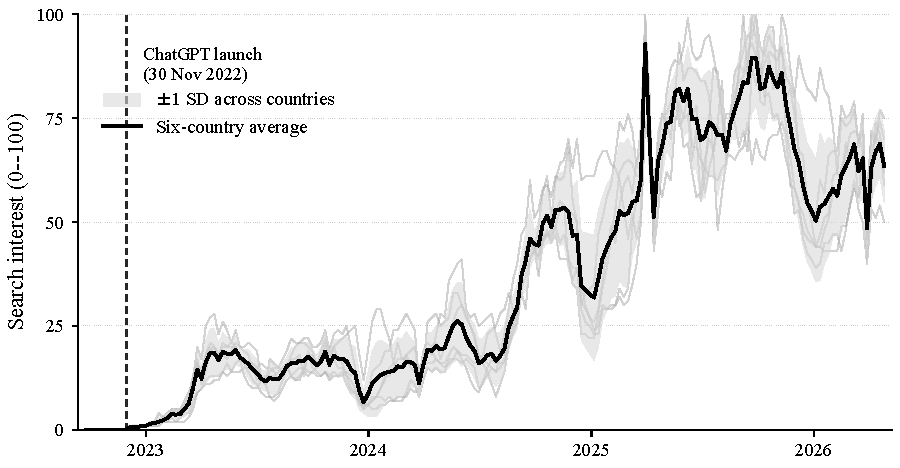
\includegraphics[width=0.85\textwidth]{fig1_chatgpt_intro.pdf}
  \end{center}
  \vspace{-0.3em}
  \footnotesize Interés de búsqueda en Google Trends para ``ChatGPT'' en seis países (CR, CO, EC, MX, PE, UY).
  Pre-lanzamiento $\approx 0$; post-lanzamiento se estabiliza entre 40 y 90.
\end{frame}

% --- Slide 5: Por que importa America Latina --------------------------------
\begin{frame}{¿Por qué América Latina?}
  La región presenta una configuración estructural \emph{opuesta} a la danesa:
  \vfill
  \begin{itemize}
    \setlength\itemsep{0.5em}
    \item \textbf{Informalidad alta:} 55\% en promedio regional, entre 25\% (Uruguay) y más de 70\% (Andinos).
    \item \textbf{Mercados laborales segmentados:} formal e informal con instituciones de fijación salarial distintas.
    \item \textbf{Adopción heterogénea:} firmas multinacionales despliegan software aumentado con LLM, pero el uso directo de ChatGPT está rezagado.
    \item \textbf{Exposición previa documentada:} \citet{Azuara2024_idb_ai}, \citet{Ciaschi2025_distributive_ai}, \citet{EganadelSol2025_ai_lac} estiman \emph{exposición potencial}, no efectos causales realizados.
  \end{itemize}
  \vfill
  \textbf{Brecha:} se ha medido la exposición; no se ha medido el efecto.
\end{frame}

% =============================================================================
\section{Contribución}
% =============================================================================

% --- Slide 6: Contribucion --------------------------------------------------
\begin{frame}{Contribución del paper}
  \begin{enumerate}
    \setlength\itemsep{0.4em}
    \item \textbf{Primera evidencia causal} de exposición a LLM sobre resultados laborales en América Latina.
    \item \textbf{DiD con tratamiento continuo} (\citet{CallawayCGBS2024_continuous}) aplicado país por país; la literatura previa usa cortes binarios.
    \item \textbf{Formalidad de línea base} elevada de subgrupo a margen central de heterogeneidad, evitando el problema del control post-tratamiento.
    \item \textbf{Crosswalk y panel reproducible} para seis países (2021--2025); insumo para futura investigación regional.
    \item \textbf{Cuatro narrativas precomprometidas} antes de correr el análisis: la narrativa enfatizada queda determinada por la evidencia, no por búsqueda \emph{ex post}.
  \end{enumerate}
  \vfill
  \textbf{Contraste central:} \citet{HumlumVestergaard2025_llm} (Dinamarca) vs.\ seis estimaciones independientes en ALC.
\end{frame}

% =============================================================================
\section{Marco teórico}
% =============================================================================

% --- Slide 7: Marco teorico (tareas) ----------------------------------------
\begin{frame}{Marco teórico: ocupaciones como conjuntos de tareas}
  Siguiendo \citet{AcemogluAutor2011_tasks} y \citet{AcemogluRestrepo2018_race}:
  \vfill
  \begin{itemize}
    \setlength\itemsep{0.5em}
    \item Cada ocupación $o$ es un conjunto de tareas $j \in [0, N]$ con pesos $s_{oj}$.
    \item El salario en la ocupación $o$ es:
      \[
        w_o = \sum_j s_{oj} \cdot p_j,
      \]
      donde $p_j$ es el precio de la tarea (depende de productividad humana y demanda).
    \item Pre-LLM: todas las tareas son realizadas por trabajo humano.
    \item Post-LLM: un subconjunto de tareas $J^{LLM}$ pasa a ser automatizable mediante software basado en LLM.
  \end{itemize}
\end{frame}

% --- Slide 8: Displacement vs Reinstatement ---------------------------------
\begin{frame}{Dos fuerzas opuestas}
  La medida de exposición de \citet{Eloundou2023_gpt_exposure} captura:
  \[
    \beta_o \;=\; \sum_{j \in J^{LLM}} s_{oj}
  \]
  \vfill
  Sobre el salario operan \emph{dos efectos}:
  \begin{itemize}
    \setlength\itemsep{0.5em}
    \item \textbf{Desplazamiento ($\tau_d$):} las tareas $j \in J^{LLM}$ pasan a hacerse con software a menor costo. Reduce la demanda por trabajo humano. Magnitud proporcional a $\beta_o$.
    \item \textbf{Reposición ($\tau_r$):} las firmas crean tareas complementarias nuevas (supervisión, ingeniería de prompts, verificación) que humanos realizan junto al software.
  \end{itemize}
  \vfill
  Efecto neto:
  \[
    \Delta w_o \;=\; (\tau_r - \tau_d) \cdot \beta_o.
  \]
  \emph{Signo y magnitud son empíricos.}
\end{frame}

% --- Slide 9: Canal de formalidad -------------------------------------------
\begin{frame}{El canal de formalidad}
  La adopción de software aumentado con LLM requiere \emph{inversión a nivel de firma}: licencias, integración, capacitación, soporte.
  \vfill
  \begin{itemize}
    \setlength\itemsep{0.5em}
    \item \textbf{Sector formal:} firmas con capital y crédito \emph{adoptan}.
    \item \textbf{Sector informal:} firmas pequeñas y descapitalizadas \emph{no adoptan}.
    \item Predicción inmediata: efectos directos del LLM se concentran en el sector formal.
    \item \textbf{Pero hay un canal indirecto:} firmas formales más productivas pueden ganar cuota de mercado a costa de las informales.
  \end{itemize}
  \vfill
  \textbf{Implicancia:} el efecto neto sobre trabajadores informales puede no ser cero, aunque la adopción directa sea cero.
\end{frame}

% --- Slide 10: Predicciones testables ---------------------------------------
\begin{frame}{Cuatro predicciones testables}
  \small
  \begin{itemize}
    \setlength\itemsep{0.45em}
    \item[\textbf{P1.}] \emph{(Cross-ocupacional, intra-país)} El signo de $\partial Y_{ot}/\partial \beta_o$ es empírico:
      desplazamiento dominante $\Rightarrow$ efecto negativo;
      reposición dominante $\Rightarrow$ efecto positivo.
    \item[\textbf{P2.}] \emph{(Formal vs informal, intra-país)} En el corto plazo,
      $|\tau^{F}| > |\tau^{I}|$ por adopción concentrada en el sector formal.
    \item[\textbf{P3.}] \emph{(Cross-país)} Países con mayor formalidad e infraestructura digital exhiben $|\tau|$ mayores.
    \item[\textbf{P4.}] \emph{(Heterogeneidad por habilidad)} Dentro de una ocupación, trabajadores con educación terciaria sufren menor desplazamiento que aquellos con educación secundaria.
  \end{itemize}
  \vfill
  \normalsize
  Las cuatro predicciones se pueden contrastar para cada uno de los seis países por separado.
\end{frame}

% =============================================================================
\section{Datos}
% =============================================================================

% --- Slide 11: Seis paises --------------------------------------------------
\begin{frame}{Datos: seis países, 2021T1--2025T4}
  \small
  \begin{tblr}{
    colspec = {l l l l},
    row{1} = {font=\bfseries},
    rowsep = 3pt
  }
  \toprule
  País       & Encuesta  & Frecuencia      & Cobertura \\
  \midrule
  Costa Rica & ECE       & Trimestral      & Nacional \\
  Colombia   & GEIH      & Mensual $\to$ T & Nacional \\
  Ecuador    & ENEMDU    & Mensual $\to$ T & Nacional \\
  México     & ENOE      & Trimestral      & Nacional \\
  Perú       & ENPE      & Trimestral      & Lima Metropolitana \\
  Uruguay    & ECH       & Anual           & Nacional \\
  \bottomrule
  \end{tblr}
  \vfill
  \footnotesize
  \textbf{Selección:} cinco países publican microdatos directamente en ISCO-08; México publica en SINCO con \emph{crosswalk} oficial a ISCO-08.
  \textbf{Caveat de Perú:} la ENAHO descontinuó el módulo trimestral de empleo en 2023; la ENPE solo cubre Lima Metropolitana, por lo que $\hat\tau^{Per\acute{u}}$ se interpreta como Lima-específico, no nacionalmente representativo.
\end{frame}

% --- Slide 12: Variable de tratamiento --------------------------------------
\begin{frame}{Variable de tratamiento: la exposición $\beta$}
  \small
  De \citet{Eloundou2023_gpt_exposure}, tres puntajes ocupacionales:
  \begin{itemize}
    \setlength\itemsep{0.3em}
    \item $\alpha_o$: sustitución directa por LLM ($\geq 50\%$ tiempo de tarea).
    \item $\beta_o$: alcanzable mediante software construido sobre LLM.
    \item $\zeta_o = \alpha_o + \beta_o$: cota superior.
  \end{itemize}
  \vfill
  \normalsize
  \textbf{Uso $\beta$ como tratamiento principal} (no $\zeta$):
  \begin{itemize}
    \setlength\itemsep{0.3em}
    \item Captura el canal dominante en ALC: software empresarial aumentado con LLM (CRM, contabilidad, atención al cliente).
    \item Más conservador que $\zeta$.
    \item $\alpha$ y $\zeta$ se reportan como exposiciones alternativas en la robustez.
  \end{itemize}
  \vfill
  \textbf{Crosswalk:} O*NET $\to$ ISCO-08 (4 dígitos), tasa de coincidencia 98.2\%.
\end{frame}

% =============================================================================
\section{Estrategia de identificación}
% =============================================================================

% --- Slide 13: Especificacion principal -------------------------------------
\begin{frame}{Especificación principal}
  Para cada país $c$ por separado:
  \[
    Y_{ot}^{c} \;=\; \tau^{c}\,\bigl(\beta_o \cdot \text{Post}_t\bigr) \;+\; \alpha_o^{c} \;+\; \alpha_t^{c} \;+\; \mathbf{X}_{ot}^{c\prime}\boldsymbol{\gamma}^{c} \;+\; \varepsilon_{ot}^{c}
  \]
  \vfill
  \begin{itemize}
    \setlength\itemsep{0.4em}
    \item Unidad: ocupación $\times$ trimestre dentro del país.
    \item $\beta_o$: continua, $\in [0, 1]$.
    \item $\text{Post}_t = \mathds{1}[t \geq 2023\text{T1}]$. Fecha común a los seis países (lanzamiento de ChatGPT, 30 nov.\ 2022; 2022T4 descartada como buffer).
    \item $\alpha_o^c, \alpha_t^c$: efectos fijos de ocupación y de tiempo dentro de cada país.
    \item Estimador: \citet{CallawayCGBS2024_continuous} para tratamiento continuo (ACRT).
    \item \emph{Clustering} a nivel ocupación; \emph{wild cluster bootstrap} cuando aplique.
  \end{itemize}
\end{frame}

% --- Slide 14: Identificacion -----------------------------------------------
\begin{frame}{Supuestos de identificación y defensa}
  \small
  \begin{itemize}
    \setlength\itemsep{0.5em}
    \item \textbf{Tendencias paralelas} (ocupaciones expuestas vs.\ no expuestas pre-shock):
      \begin{itemize}
        \item Test de pre-tendencias gráfico (\emph{event study}).
        \item Cotas Honest-DiD de \citet{RambachanRoth2023_honest} elevadas a identificación principal.
        \item Placebos transversales sobre ocupaciones con $\beta = 0$.
      \end{itemize}
    \item \textbf{No anticipación:} ChatGPT exógeno a mercados laborales latinoamericanos; pre-acceso restringido a empleados de OpenAI.
    \item \textbf{SUTVA:} \emph{spillovers} dentro de firma discutidos y acotados.
    \item \textbf{Exogeneidad de la exposición:} O*NET es un atributo predeterminado de tareas (Estados Unidos), no un \emph{outcome} de los mercados laborales latinoamericanos.
  \end{itemize}
  \vfill
  \normalsize
  \textbf{Nota:} placebos temporales (2019, 2021) no son factibles en muestra post-COVID. Se reemplazan por placebos transversales y \emph{outcomes} placebo (horas semanales de trabajadores agrícolas manuales).
\end{frame}

% --- Slide 15: Heterogeneidad -----------------------------------------------
\begin{frame}{Heterogeneidad: formalidad de línea base}
  \textbf{Problema:} la formalidad contemporánea es ella misma un \emph{outcome} de la exposición a LLM (\emph{bad control}, \citet{AbadieAIW2023_cluster}).
  \vfill
  \textbf{Solución:} uso la formalidad de línea base $F_{i, 2021}$ como variable de interacción primaria.
  \vfill
  Especificación:
  \[
    Y_{ict} = \tau\beta_o \text{Post}_t + \delta\,(\beta_o \text{Post}_t F_{i,2021}) + \alpha_o + \alpha_t + \varepsilon
  \]
  \vfill
  Otras dimensiones de heterogeneidad pre-registradas: género, edad, educación, sector, urbano/rural.
\end{frame}

% --- Slide 16: Robustez -----------------------------------------------------
\begin{frame}{Capa de robustez}
  \small
  \begin{itemize}
    \setlength\itemsep{0.35em}
    \item Cotas Honest-DiD ($\bar M$) de \citet{RambachanRoth2023_honest}.
    \item Especificaciones binarias alternativas: cutoff $p50$ (siguiendo a \citet{Liu2025_generate_future}) y cutoff teórico $\beta > 0.5$.
    \item Medidas de exposición alternativas: $\alpha$, $\zeta$, \citet{Webb2020_ai_exposure}, \citet{Felten2023_ai_exposure}.
    \item Diseño Bartik / \emph{shift-share} con shares de empleo de 2021 (\citet{GoldsmithPinkham2020_bartik}, \citet{BorusyakHJ2022_shiftshare}).
    \item Cotas de \citet{Oster2019_unobservables} para selección sobre no observables ($\delta = 1$, $R^2_{\max} = 1.3 \cdot R^2$).
    \item Múltiples comparaciones: Romano-Wolf intra-dimensión + Bonferroni entre dimensiones.
    \item Drop-one ocupación, drop-one país, fallback a 3 dígitos ISCO-08, \emph{wild cluster bootstrap}.
  \end{itemize}
\end{frame}

% =============================================================================
\section{Narrativas y estado}
% =============================================================================

% --- Slide 17: Cuatro narrativas --------------------------------------------
\begin{frame}{Cuatro narrativas precomprometidas}
  Para cada país, una de cuatro narrativas resultará compatible con los datos:
  \vfill
  \small
  \begin{itemize}
    \setlength\itemsep{0.45em}
    \item[\textbf{A.}] \textbf{Informalidad amplifica:} $|\hat\tau^c| > 2\%$, impulsado por canal informal ($\tau_I^c < \tau_F^c < 0$).
    \item[\textbf{B.}] \textbf{Replicación del nulo ALC--Dinamarca:} efectos a nivel país indistinguibles de cero en ambos canales.
    \item[\textbf{C.}] \textbf{Nulo en formal, grande en informal:} $\tau_F^c \approx 0$, $\tau_I^c$ negativo y significativo. Identifica un canal que diseños daneses y estadounidenses no detectan.
    \item[\textbf{D.}] \textbf{Ganancias estratificadas:} efectos salariales positivos en trabajadores formales urbanos con educación terciaria, sin efecto sobre la mayoría informal.
  \end{itemize}
  \vfill
  \normalsize
  \textbf{Compromiso \emph{ex ante}:} la narrativa enfatizada queda determinada por el patrón observado, no por búsqueda \emph{ex post} de especificación.
\end{frame}

% --- Slide 18: Estado del proyecto ------------------------------------------
\begin{frame}{Estado actual del proyecto}
  \begin{itemize}
    \setlength\itemsep{0.45em}
    \item[\textbf{Hecho.}]
      \begin{itemize}
        \item Estrategia de identificación finalizada y validada.
        \item Crosswalk O*NET $\to$ ISCO-08 construido (98.2\% match).
        \item Datos crudos de los seis países descargados, descomprimidos y normalizados (127 GB).
        \item Borrador del paper en español: introducción, marco teórico, metodología.
      \end{itemize}
    \item[\textbf{En curso.}]
      \begin{itemize}
        \item Armonización de microdatos: 6 encuestas con esquema común.
        \item Imputación de exposición $\beta$ a microdatos por país.
      \end{itemize}
    \item[\textbf{Pendiente.}]
      \begin{itemize}
        \item Estimación principal país por país.
        \item Robustez: Honest-DiD, Bartik, Oster, alternative exposures.
        \item Sección de resultados, sección de robustez, conclusión.
      \end{itemize}
  \end{itemize}
\end{frame}

% --- Slide 19: Preguntas para el asesor -------------------------------------
\begin{frame}{Preguntas para discutir}
  \begin{enumerate}
    \setlength\itemsep{0.5em}
    \item \textbf{Estimador principal:} ¿continuous DiD (CGBS 2024) o TWFE simple? Trade-off entre frontera metodológica y comparabilidad con la literatura cercana.
    \item \textbf{Caveat de Perú:} ¿incluir Perú con representatividad solo de Lima, o relegarlo a robustez? La justificación está en el diseño de la ENPE.
    \item \textbf{Cutoff binario para la especificación secundaria:} mediana ($p50$) por comparabilidad con \citet{Liu2025_generate_future} vs.\ cutoff teórico de $\beta > 0.5$.
    \item \textbf{Posicionamiento del paper:} ¿énfasis en contraste con Dinamarca o en las cuatro narrativas como contribución metodológica?
    \item \textbf{Journal objetivo:} JLE, JHR, AEJ:Applied. Calendario de presentaciones previas (LACEA, NEUDC, IZA).
  \end{enumerate}
\end{frame}

% --- Slide 20: Gracias ------------------------------------------------------
\begin{frame}[plain]
  \begin{center}
    \vspace{1cm}
    {\Large \textbf{Gracias.}}\\[1.5em]
    {\large Comentarios bienvenidos.}\\[2cm]
    {\small Eric Torres \\ \texttt{etorres@pucp.edu.pe}}
  \end{center}
\end{frame}

\end{document}
